\section{Einleitung}
\label{sec:Einleitung}

Neben der Bestrahlung der Fersensporn wird die Strahlentherapie auch bei anderen Krankheitsbildern eingesetzt. In diesem Fall handelt es sich wieder um einen orthopädischen Fall und es geht um ein Befund der linken Hüfte (Bursitis trochanterica). 

\section{Patientenvorstellung}
\label{sec:Vorstellung}

Seit Mai 2015 hat die Patienten Beschwerden an der linken Hüfte. Zur Linderung der Symptome gab es eine Spritzentherapie und es wurden ihr NSAR verabreicht. Diese konservativen Therapiemaßnahmen haben keinen Erfolg gezeigt und der Patientin wurde indiziert zur Linderung der Symptome bestrahlt zu werden. Außerdem wurden ihr auch die möglichen Wirkungen und Nebenwirkungen der Strahlentherapie erklärt. Zur weiteren Diagnosen gehört vor allem eine Schilddrüsenunterfunktion und Hypercholesterinämie. Sie ist $\SI{160}{\centi\meter}$ groß und hat ein Gewicht von $\SI{60}{\kilo\gram}$. Die lateralen Druckschmerzen befinden sich an der linken Hüfte. Für die Bestrahlungsplanung gehört eine Gesamtdosis von $\SI{3}{\gray}$, welche in Fraktionen von $\SI{0,5}{\gray}$ in insgesamt 6 Bestrahlungen appliziert werden soll. Insgesamt sollen 3 Bestrahlungen pro Woche stattfinden. Das soll dabei helfen, dass der Körper genug Zeit hat, auf die Behandlung zu reagieren. Fall es nach 8-10 Wochen keine Besserung ergibt, muss die Bestrahlung wiederholt werden.

\section{Bestrahlungsplanung}
\label{sec:bestrahlung}

Das PTV ist in den CT-Daten bereits eingezeichnet und als nächstes wurde die Kontur der Hüfte als Body-Struktur eingezeichnet. Andere Gegenstände, wie z.B. Lagerungshilfe oder Patientenliege, werden auch als Struktur eingezeichnet, weil sich diese auch im Strahlengang befinden. Dosiert wird hier auf den ICRU Referenzpunkt und das Ziel der Bestrahlungsplanung ist, dass das Planungszielvolumen durch die $\SI{95}{\percent}$ Isodosenlinie umschlossen wird. Das Dosismaximum soll bei $\SI{115}{\percent}$ liegen. Für die Bestrahlungsplanung wurden zwei Felder mit einer Gewichtung von 0.5 erzeugt. Die beiden Felder sind gleich groß und zwar beide haben eine Größe von  $\SI{14}{\centi\meter}$ x $\SI{11.5}{\centi\meter}$. Beim ersten Feld gibt es eine Gantry-Rotation von $0^\circ$ und beim zweiten eine Gantry-Rotation von $180^\circ$. Der Bestrahlungsplan wird auf "$\SI{100}{\percent}$ target mean" normiert. Für die Schonung des umliegenden Gewebes werden MLCs verwendet, die an die Struktur angepasst werden können. Das ist in der Abbildung \ref{fig:kombi} zu sehen. 

\begin{figure}[htpb]
	\centering
	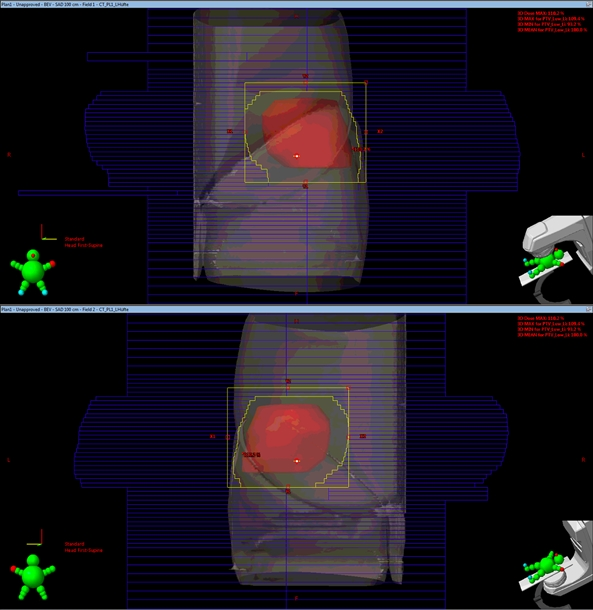
\includegraphics[width=0.7\linewidth]{../Bilder/kombi}
	\caption{Zu sehen ist die Darstellung der Lamellen. Beim oberen Bild handelt es sich um das Feld bei $0^\circ$ und beim unteren Bild handelt es sich um das Feld bei $180^\circ$.}
	\label{fig:kombi}
\end{figure}
